\begin{frame}{Nonnegative rank}
\begin{defn}[Nonnegative rank]
Given $X \in \mathbb{R}_+^{p\times n}$, the nonnegative rank of X, denoted $\text{rank}_+(X)$ is the minimum $r$ s.t. $\exists W \in \mathbb{R}_+^{p\times r}, H \in \mathbb{R}_+^{r\times n} \text{ with } X = WH$.
\end{defn}
\centering
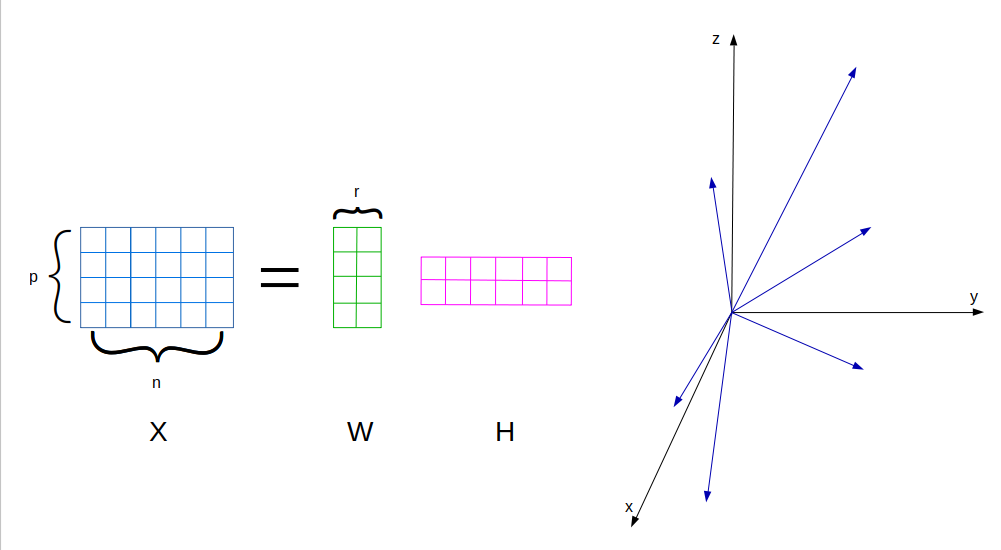
\includegraphics[scale=0.28]{../images/NMFvect.png}
\end{frame}
\begin{comment}
\begin{frame}{Computational Geometry : Nested polytopes problem}
\begin{figure}
\centering
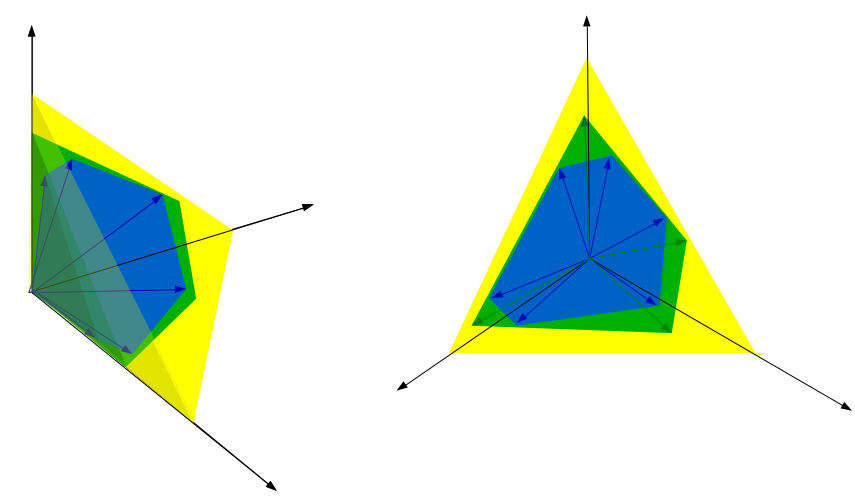
\includegraphics[scale=0.35]{../images/polytopeGeo.png}
\caption{\footnotesize Finding a polytope with minimum nb of vertices nested between 2 polytopes}
\end{figure}
\end{frame}
\end{comment}
\begin{frame}{Graph Theory : Bipartite dimension}
Let $G(X) = (V_1 \cup V_2, E)$ be a bipartite graph induced by X (i.e. $(i,j)\in E \Leftrightarrow X_{ij}\neq 0$).
\begin{defn}[Biclique and bipartite dimension]
\begin{itemize}
\item A biclique (or a complete bipartite graph) is a bipartite graph s.t. every vertex in $V_1$ is connected to every vertex in $V_2$. 
\item The bipartite dimension (or the minimum biclique cover) bc$(G(X))$ is the minimum number of bicliques needed to cover all edges in E.
\end{itemize} 
\end{defn}

\end{frame}

\begin{frame}

\begin{figure}
\centering
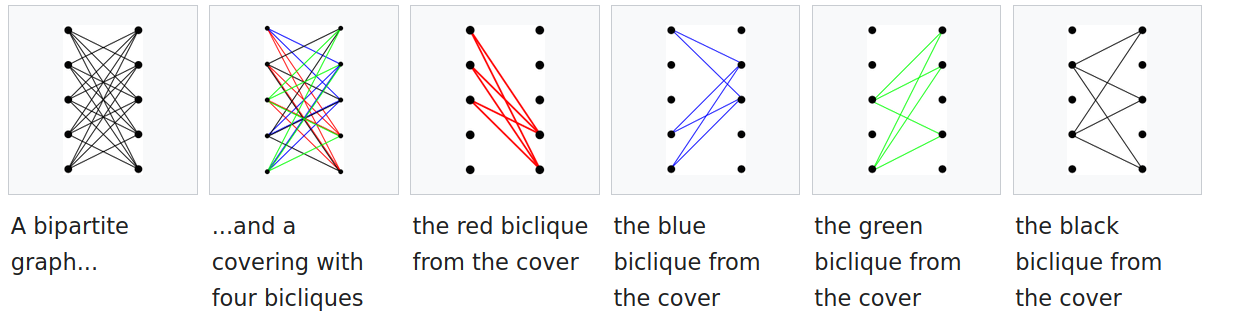
\includegraphics[scale=0.2]{../images/biclique.png}
\caption{Example for biclique edge cover \cite{biclique}}
\end{figure}
\begin{comment}
For any $(W,H)\geq 0$ s.t. $X = WH = \sum_{k=1}^r W_{:k}H_{k:} := \sum_{k=1}^r X_k$, we have 
\[G(X) = \cup_{k=1}^r G(W_{:k}H_{k:})
\]
where $G(W_{:k}H_{k:})$ are complete bipartite subgraphs (bc$(G(W_{:k}H_{k:}) = 1 \forall k$).
\end{comment}
\begin{thm}[Rectangle covering bound]
\[\text{bc}(G(X))\leq \text{rank}_+(X)
\]
\end{thm}
\end{frame}
\begin{comment}
\begin{frame}{Communication complexity}
\begin{center}
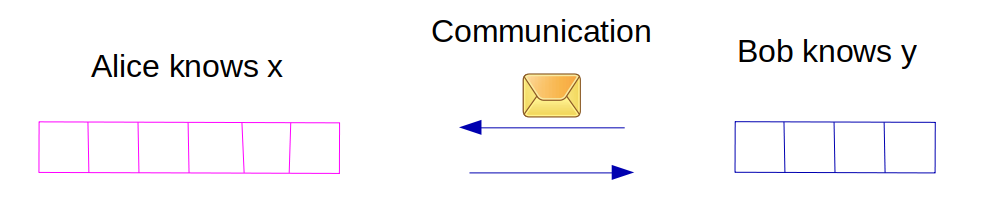
\includegraphics[scale=0.2]{../images/communication.png}
\end{center}
\small
Alice and Bob want to compute :
\[f:\{0,1\}^m \times \{0,1\}^n \rightarrow \{0,1\} : (x,y) \rightarrow f(x,y)
\]
While minimizing the nb of bits exchanged (i.e. communication complexity (CC)).


\textbf{Nondeterministic comm. complex. of $f$ (NCC)}: CC of $f$ with oracle/ message before starting the communication.


The communication matrix $X \in \{0,1\}^{2^n\times 2^m}$ is equal to the function $f$ for all possible combinations of inputs.

\begin{thm}[Yannakis]
\[\text{NCC of } f \leq \log_2(\text{rank}_+(X))
\]
\end{thm}
\end{frame}
\end{comment}
\begin{frame}{Linear Optimization : Extended formulation}
\begin{align*}
\text{(LP) } & \max & c^T x\\
 &s.t. & Ax\leq b\\
 & & x \in \mathbb{R}^n \geq 0
\end{align*}
\begin{defn}[Extended formulation]
The extended formulation of a polytope P is a higher dimensional polytope Q and a linear projection $\pi$ s.t. $\pi(Q) = P$.
\end{defn}
In our LP problem, an extended formulation of the polytope $P \subset \mathbb{R}^n$ defined by the constraints $Ax\leq b$, is a polytope $Q\subset \mathbb{R}^{n+r}$ defined by $Cx+Dy \leq d$ with $y\in \mathbb{R}^r$, s.t. $\pi(Q) = P$.

\end{frame}

\begin{frame}
The slack matrix $X(i,j) = b_i-A_iv_j$.

With $v_j$, the $j^{th}$ vertex of P and $\{x\in \mathbb{R}^n | b_i-A_ix\geq 0\}$ its $i^{th}$ facet.

The (i,j) entry measures the slack of the $i^{th}$ inequality for the $j^{th}$ vertex. 
\begin{thm}[Yannakis]
The minimum size of an extended formulation Q of P is equal to $\text{rank}_+(X)$.
\end{thm}

When P has exponentially many facets, finding extended formulations allows to solve the LP in polynomial time.
\end{frame}